\chapter{Wykład 10. Zarządzanie kosztami w projekcie informatycznym}

\section{Plan poprawy procesu}
% strona 23

\textbf{I. Opracuj: plan poprawy procesu.}

\begin{enumerate}
\item Zapoczątkowanie poprawy procesu.
\begin{enumerate}

\item Definicja kontekstu oraz budżetu (sponsorowania) programu.
\item Ustalenie infrastruktury niezbędnej do doskonalenia procesu.
\end{enumerate}


\item Ocena dotychczas stosowanego procesu.
\item Identyfikacja obszarów procesu, które będą doskonalone.
\begin{enumerate}

\item Definicja strategii doskonalenia.
\item Podział zadań - "co, kto, jak i kiedy".
\item Implementacja procedury doskonalenia procesu.
\end{enumerate}


\item Zbadanie efektów procedury doskonalenia procesu.
\begin{enumerate}

\item Ponowna ocena procesu (w ograniczonym zakresie).
\item Analiza wyników początkowej oceny procesu z ponowną jego oceną.
\end{enumerate}

\item Walidacja procedury doskonalenia procesu wytwórczego.
\begin{enumerate}

\item Utrzymanie tempa i wyników procedury doskonalenia.
\item Formalne wprowadzenie procedury poprawy procesu do misji organizacji.

\end{enumerate}
\end{enumerate}



textbf{II.Wyznacz TCO i ROI.}

Koszty początkowe:
\begin{itemize}

\item kupno nowego sprzętu komputerowego – 4 000 zł,
\item koszty serwera do wersjonowania – 10 000 zł.
\end{itemize}

Koszty coroczne:
\begin{itemize}

\item serwis sprzętu – 1 000 zł,
\item cotygodniowe sprawdzanie i robienie backupów – 6 000zł.
\end{itemize}

Koszt przez  5 lat to 49 000 zł.
TCO rocznie:  9 800 zł.
\textbf{TCO miesięcznie:  817 zł.}
Przychód początkowy:
\begin{itemize}

\item szkolenie załogi - Koszt szkolenia 10 000 zł,
\item sprzedaż programu – 25 000 zł.
\end{itemize}

Przychód coroczny:
\begin{itemize}

\item przychód  z licencji - 7 000 zł,
\item serwis i upgrady – 10 000 zł.
\end{itemize}

Przychód wypracowany przez 5 lat: 120 000 zł.
Przychód rocznie : 24 000 zł.
Przychód miesięcznie: 2000 zł.
\textbf{Zysk netto: 2 000 zł – 817 zł = 1183 zł.}
\textbf{ROI:  1183\backslash817 * 100\% = 144,8\%} 

% ===========================================================================

\section{Plan zarządzania kosztami}
% strona 26

\textbf{I. Opracuj plan zarządzania kosztami.}

Zarządzanie kosztami:
\begin{enumerate}
\item Planowanie zasobów:
\begin{enumerate}
\item Struktura podziału pracy – opinie ekspertów.
\item Dane historyczne – określenie różnych wariantów realizacji.
\item Deklaracja zakresu – oprogramowanie wspierające zarządzanie projektami.
\item Opis puli zasobów.
\item Procedury organizacyjne.
\item Szacunki czasu trwania działań.
\end{enumerate}

\item Szacowanie kosztów:
\begin{enumerate}

\item WBS – szacowanie porównawcze.
\item Wymagania dotyczące zasobów – modelowanie parametryczne.
\item Ceny jednostkowe zasobów – szacowanie oddolne.
\item Szacunki czasu trwania działań.
\item Publikowane szacunki – inne metody szacowania.
\item Dane historyczne.
\item Plan kont
\item Dane o ryzykach.

\end{enumerate}

\item Budżetowanie kosztów:

\begin{enumerate}

\item Szacunki kosztów.
\item WBS.
\item Harmonogram projektu.
\item Plan zarządzania ryzykiem.

\end{enumerate}

\item Kontrola kosztów:
\begin{enumerate}
\item Plan bazowy kosztów – system kontroli zmian kosztów.
\item Raport z wykonania – pomiar wykonania.
\item Żądania zmian – technika zarządzania wartością wypracowaną.
\item Plan zarządzania kosztami – dodatkowe procesy planowania.
\end{enumerate}
\end{enumerate}



% ===========================================================================

\section{Wprowadzenie kosztów do planu projektu}
% strona 41

Tabela kosztów zaimportowana z programu MS Project:

\begin{figure}[!h]
\centering
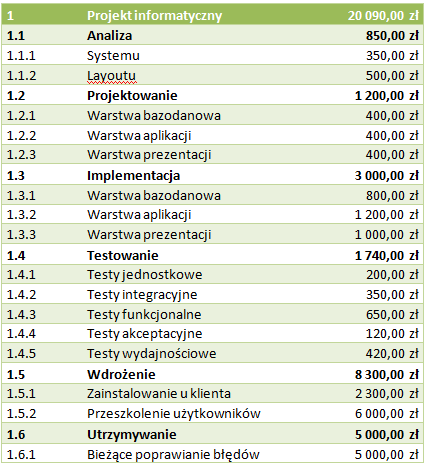
\includegraphics[width=1.1\textwidth]{tabelaKosztow.png}
\caption{Tabela kosztów}
\label{fig:tabelaKosztow}
\end{figure}

% ===========================================================================

\section{Monitorowanie projektu z wykorzystaniem EVA}
% strona 69

Poniższe wyliczenia zostały wykonane w programie MS Project, a nagłówki kolumn zostały nazwane polskimi odpowiednikami metody EVA (Earned Value Analysis) – wczesnej analizy wartości wypracowanej.

\begin{figure}[!h]
\centering
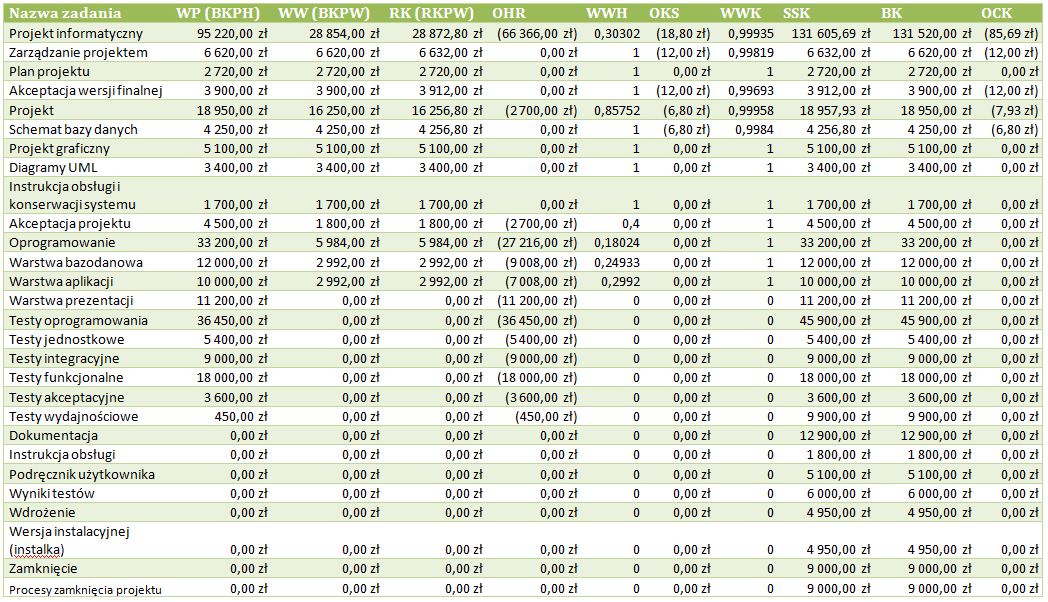
\includegraphics[width=1.1\textwidth]{monitorowanieEVA.png}
\caption{Monitorowanie projektu z wykorzystaniem EVA}
\label{fig:monitorowanieEVA}
\end{figure}
